\section{SEP Prototype}~\label{sec:prototype}

%With the purpose of demonstrating the feasibility of the proposed platform, 

%In this section, a platform prototype comprising state-of-art tools  materializing the proposed architecture and services is presented. 

%Extensions to the architecture and implementation of \textit{OpenWhisk}, an open source FaaS platform.

%, evaluating it in different aspects. 
%Figure~\ref{fig:Serverless_Edge_Platform_Overview} presets an overview of the SEP prototype containing all the proposed services. In addition to the services discussed in Section~\ref{sec:SEP}, it includes a \textit{Reverse Proxy}, which is responsible for proxying external HTTP/WebSocket requests to internal platform services.

Figure~\ref{fig:Serverless_Edge_Platform_Overview} presents the SEP architecture with the \textit{Load Balancer} part of the \textit{Controller}. Each SEP component was deployed as a Docker container; apart from the MQTT broker (Mosquitto), remaining components are either original or extended versions from OpenWhisk technology stack.


\subsection{OpenWhisk}

OpenWhisk~\cite{OpenWhisk} is a state-of-art tool implementing the FaaS model. Originally developed by IBM, it is now an open source project incubated by Apache. It is also the most mature open source FaaS tool available. 

OpenWhisk plays a central role in the proposed SEP architecture %First and foremost,
%as it takes care of the dynamic creation and termination of containerized environments. More precisely, 
by handling the creation and termination of \textit{Docker} containers
%\footnote{Other less popular container engines are also supported} 
with a specific runtime supporting the execution of stateless functions. Functions are activated by rules associated with triggers, which in turn are mapped to internal and external events, including HTTP(S) requests. %TODO: activations, syncrhonous and asynchronous requests

OpenWhisk features a service-oriented architecture.
Among others, it comprises the following components~\cite{OpenWhisk}:

\begin{itemize}

    \item \textit{Nginx}: a multi-purpose tool featuring a \textit{reverse proxy}; this component enables the external invocation of the platform \textit{API}, including the upload and triggering of \textit{functions};
    
    \item \textit{Controller}: responsible for validating, authenticating, and distributing (load balancing) requests to \textit{Invokers}; and 
    
    \item \textit{Invoker}: responsible for the management of a pool of CERs, including their creation upon function invocation and termination upon a period of idleness;
    
    
    %selecting or creating a CER for the execution of a function activation.
    
\end{itemize}

\subsection{Latency-Sensitive Computation Offloading}

%TODO ETSI comparison
%TODO define MEC
To cope with the requirements of latency-sensitive computation offloading, SEP components are deployed to fog nodes in close proximity with end-users
(e.g., cloudlets or MEC nodes). In this configuration, client devices interface with  OpenWhisk's \textit{Controller} through its \textit{Reverse Proxy} (Nginx).

%the critical path that starts with the client request and finishes with the response notification must remain near the edge. 


Depending on the installed capabilities, OpenWhisk's \textit{Invoker} can be deployed to one or multiple VMs. Each \textit{Invoker} takes care of a pool of containers whose maximum size depends on the available resources. The load is distributed among \textit{invokers} by OpenWhisk's \textit{Load Balancer}.
%, who monitors the health status of each \textit{Invoker}.

%OpenWhisk's \textit{Invoker} is purely event-driven. 
Upon a function invocation, the \textit{Invoker} checks for the availability of a warm (idle) CER before creating a new one. To mitigate cold start of latency-sensitive functions, the \textit{idleness time} has been increased from \textit{50~ms} to \textit{500~ms}. More robust extensions targeting a more efficient resource allocation should consider a dynamic optimization of this parameter.

OpenWhisk does not provide native support for the \textit{WebSocket} protocol. Coherently with what has been discussed in Section~\ref{sec:SEP_MCO}, we have extended OpenWhisk to enable a more efficient communication between SEPs and edge devices hosting real-time and interactive applications. 
%The proposed extension consists of the following modifications: 
%\begin{itemize}
%    \item a new endpoint entry supporting the \textit{WebSocket} protocol in \textit{Nginx}'s configuration; and
%    \item the additional implementation handling \textit{WebSocket} messages in the \textit{Controller} component.
%\end{itemize}
%upon the activation of actions --- a stateless function written in one of the many languages supported by the tool.
%OpenWhisk is implemented as an event-driven platform. 
In turn, OpenWhisk natively supports function sequences, which allow the creation and triggering of sequential execution flows using the platform's API. Our prototype exploits this feature for the definition of the \textit{Workflow Service} discussed in Section~\ref{sec:SEP_MCO}. Future extensions may consider the support of more comprehensive flow-based languages. %(e.g., from visual programming tools such as \textit{NodeRED}).

\begin{figure}[tbp]
	\centering
	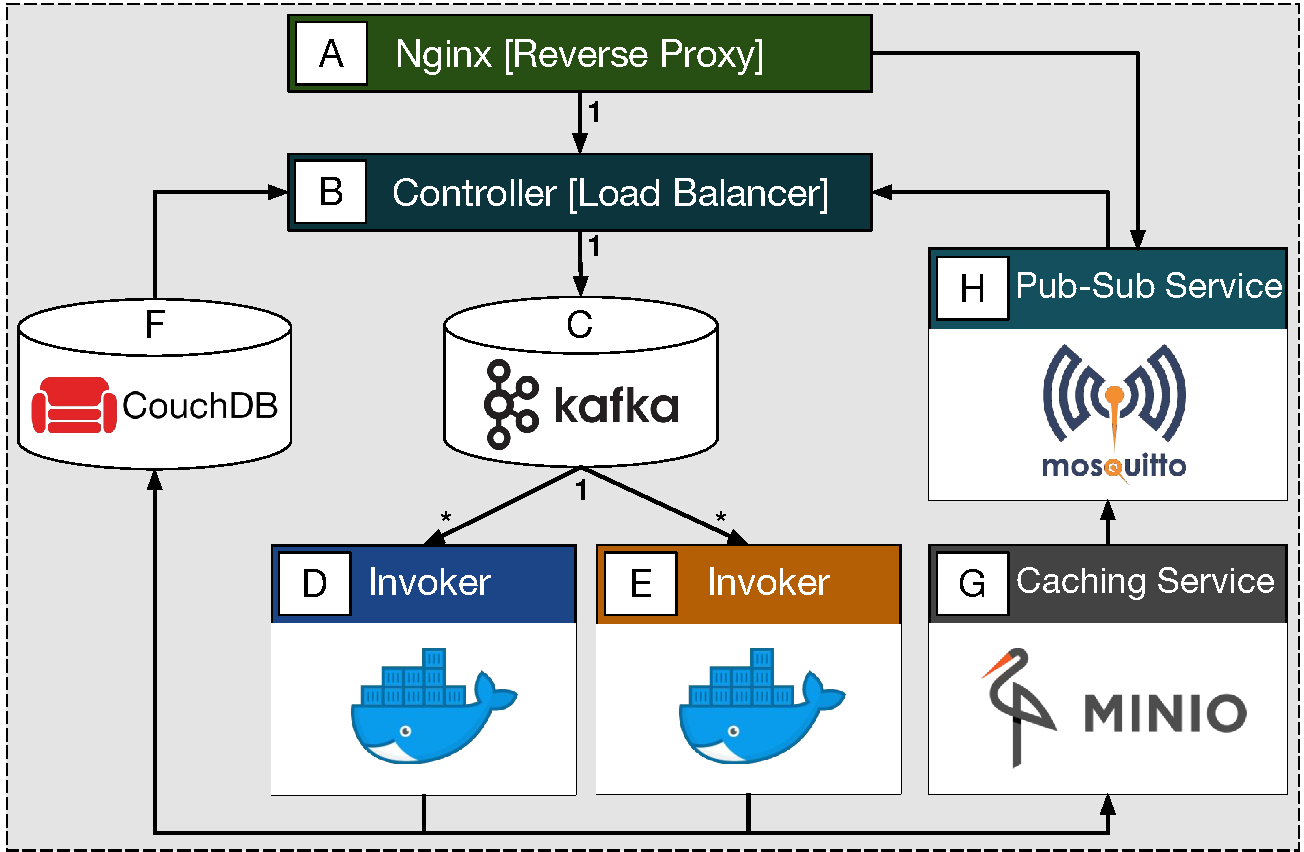
\includegraphics[width=1\linewidth]{Figs/Serverless_Edge_Platform_Prototype.pdf}
	\caption{Overview of the SEP prototype architecture}
	\label{fig:Serverless_Edge_Platform_Overview}
\end{figure}

%\subsection{Caching Service}

Finally, for the materialization of the \textit{Caching Service} discussed in Section~\ref{sec:SEP_MCO}, we adopted \textit{Minio}, an open source and lightweight object storage tool already part of OpenWhisk stack.
Minio is compatible with \textit{AWS S3} --- a state-of-art object storage service --- and features native integration with different types of notification systems and an API for managing objects. These characteristics are particularly important in the context of a SEP platform, as object events (e.g., creation, update) can trigger the execution of SEP functions, whereas functions have access to cached objects through API calls. 

%an event-driven serverless architecture

%a prototype of the caching service discussed in ~\ref{sec:SEP_MCO} was implemented as a separated module in Python language. Figure~\ref{fig:SEP_Low_Latency_FaaS} presents the resulting platform architecture.

%existing containers and an \textit{Invoker} responsible for the creation and termination of containers. 


\subsection{Opportunistic Edge Data Analysis}

OpenWhisk lacks support for the dynamic placement of functions based on latency requirements and other criteria. Nonetheless, it features a \textit{Load Balancer} that decides, among distributed \textit{Invokers}, where to send requests. 
%Each pool is interfaced and managed by an \textit{Invoker} component. 
The \textit{Load Balancer} communicates with OpenWhisk's \textit{Invoker} through messages buffered and persisted by \textit{Apache Kafka}, a high-throughput, distributed, publish-subscribe messaging system.
%(see Figure~\ref{fig:Serverless_Edge_Platform_Overview}). 

%an implementation of the \textit{Actor Model} featuring reliable queues.

To evaluate the feasibility of the opportunistic placement discussed in Section~\ref{sec:SEP_EDA}, our prototype configures OpenWhisk to be aware of two invokers: a local one mimicking an edge deployment, and another hosted by a remote node mimicking a cloud deployment. It required two interventions: 

\begin{itemize}
    \item the initialization of an external (cloud) \textit{Invoker} referencing the SEP \textit{Load Balancer}'s public IP; and
    
    \item the prioritization by the \textit{Load Balancer} of the local \textit{Invoker} whenever the response time is below a threshold. %the CPU or memory load at the SEP is below 90\%. 
\end{itemize}

The opportunistic placement prototype also required modifications from the \textit{Invoker} side. More precisely, function activation now takes as parameter the \textit{maximum number of CER instances} each function can have --- as decided by an \textit{Orchestrator}. If this limited is achieved, the function activation fails and the original request is put back into the \textit{Load Balancer} queue. As the response time increases above the threshold, requests are diverged 
%by the \textit{Load Balancer} 
to the cloud-based \textit{Invoker}. 
As discussed in Section~\ref{sec:SEP_EDA}, this configuration is suitable for SEPs in close proximity with end-users, whereas regional SEPs outside the main network path towards the cloud should rely on external load balancers. 

Finally, an \textit{Orchestrator} was implemented as a separated module in Python language. Its simple role is to monitor the arrival rate of different functions and inform the SEP for the share of resources each function may allocate. 


%or become a bottleneck in intermediary deployments (e.g., regional SEPs covering larger areas). 


%The evaluation of more sophisticated orchestration strategies is out of the scope of this work. 

%Contrasting with real-time FaaS, we further extended OpenWhisk's Load Balancer with scheduling capabilities. The idea is to take different latency requirements into account and prioritize those with more strict deadlines. For this, requests arriving at the SEP's Controller are sorted by means of a \textit{deadline first} algorithm before been distributed by the Load Balancer.

\subsection{Stateful Services}

%To address the need of stateful services, 
We have enabled stateful application partitions to run in a similar environment from stateless functions by extending OpenWhisk's \textit{Invoker}. In contrast with stateless functions --- which can be executed by any available or new CER with the corresponding runtime --- stateful services are identified by a token mapped to one specific CER upon initialization (\textit{session start event}). 

Every invocation to the stateful service is delegated to the corresponding CER by means of an \textit{update command}. This additional command specifies the service function to be performed along with any parameters from the original request. The resulting mechanism enables state to be consistently evolved at each invocation from one or distinct clients within the same session until CER termination (\textit{session end event}).

%Figure~\ref{} illustrates the stateful service life-cycle.

\subsection{Real-time Edge Coordination}

%Among the stack of technology composing OpenWhisk lies \textit{Kafka}, a high-throughput, distributed, publish-subscribe messaging system. 

The need for a publish-subscribe notification service is addressed with the adoption of \textit{Mosquitto}, an open source MQTT implementation largely adopted by IoT practitioners. %MQTT is the standard protocol for IoT machine-to-machine communication. 
Among its features, its \textit{broker} enables \textit{topic bridging} and \textit{remapping}. The former allows two or more brokers to become publish/subscribers of each other, so that messages published to one broker are propagated. In turn, topic renaming allows the definition of prefixes to the topics propagated from/to other brokers. The platform prototype exploit these features to allow the location-aware propagation of events from/to surrogate SEPs, as discussed in Section~\ref{sec:SEP_RTEC}. %Figure~\ref{} illustrates the resulting architecture.

The integration of OpenWhisk with the MQTT service requires the definition of a \textit{feed}.
OpenWhisk allows the implementation of \textit{feeds} through different architectural patterns. In particular, we used the \textit{Service Provider} pattern to keep long-lived connections to the MQTT broker. In this pattern, the \textit{Service Provider} intermediates the subscription of \textit{triggers} to MQTT topics and the invocation of those \textit{triggers} upon topic events. Each trigger can subscribe to one or more topics and activate one or more functions. The \textit{Service Provider} runs in its own container. To prevent the loss of data, each trigger subscription is persisted to the SEP NoSQL database (\textit{CounchDB}).


%To prevent bottleneck, the \textit{Service Provider} must cope with the flow of events from the MQTT broker. by distributing subscriptions among multiple service instances.
%A robust implementation must also persist trigger subscriptions in a reliable way (e.g., by using the SEP NoSQL database).


\subsection{Nginx}\label{sec:prototype_Nginx}

Last but not least, SEPs should interface with the external world by means of a gateway. Its role is to map external invocations (e.g., HTTP, WebSocket) to the platform services. %(e.g., FaaS, publish-subscribe system, etc). 

Nginx is a state-of-art tool open source tool featuring, among others, a reverse proxy. This tool is also natively integrated with OpenWhisk. 
%It allows the specification of endpoints that are mapped to internal applications. 
Due to its maturity and popularity, we adopted Nginx in our SEP prototype.

%\subsection{SEP Product Line}

%TODO: contextualize the paragraph below
%Figure~\ref{} represents the serverless edge platform as a software product line~\cite{} with product variants targeting different types of edge infrastructure and application scenarios.
